\documentclass[UTF8]{ctexart}
\usepackage{anyfontsize}  %去除ctex字體報錯
\usepackage{amsmath}
\usepackage{amssymb} 
\usepackage{extarrows}
\usepackage{titlesec}
\usepackage{titletoc}

\usepackage{pgf}
\usepackage{tikz} % Required for drawing custom shapes
\usetikzlibrary{shapes,backgrounds,arrows,automata}
% \usetikzlibrary{arrows,backgrounds}
% \usepackage{tikz}

\usepackage{geometry}
\usepackage{fancyhdr}
\usepackage{setspace}
\usepackage{indentfirst}
\usepackage{booktabs}

% \usepackage{ctex}
\usepackage{listings}

\lstdefinestyle{v1}{
language={C},
basicstyle=\scriptsize\tt,
% basicstyle=\footnotesize\tt,
keywordstyle=\color{blue}\bfseries,
stringstyle=\color{green!50!black},
identifierstyle=\color{yellow!60!black},
showstringspaces=false,
commentstyle=\color{gray},
% backgroundcolor=\color[RGB]{245,245,244},
frameround = tttt,
% frame=shadowbox,
% frame=lines,
frame=single,
tabsize=2,
xleftmargin=2cm, 
xrightmargin=2cm,
rulecolor=\color{gray},  
rulesepcolor=\color{gray}  
} 

\newcommand{\ms}[1]{
    \begin{small}
        #1
    \end{small}
}




 
\renewcommand{\headrulewidth}{0pt}  
\renewcommand{\footrulewidth}{0pt}  
\renewcommand{\headwidth}{\textwidth}

% \newcommand{\ma}[1]{\begin{array}{llll} #1 \end{array}}
% \newcommand{\mb}[1]{\textbf{#1}}
% \newcommand{\meq}[2]{\xlongequal[#2]{#1}}
% \newcommand{\mt}[1]{\text{#1}}
% \newcommand{\p}{\par}
 



\newcommand{\Rmnum}[1]{\uppercase\expandafter{\romannumeral #1}} 
\newcommand{\mR}[1]{\uppercase\expandafter{\romannumeral #1}} 
\newcommand{\mt}[1]{\text{#1}}
\newcommand{\mb}[1]{\textbf{#1}}
\newcommand{\md}[1]{\displaystyle{#1}}
\newcommand{\mda}[1]{$\displaystyle{ #1 }$}
\newcommand{\mf}[1]{\left( #1\right)}
\newcommand{\mfa}[1]{\left| #1\right|}
\newcommand{\mfb}[1]{\left\{ #1\right\}}
\newcommand{\mfc}[1]{\left[ #1 \right]}
\newcommand{\mfd}[1]{ \lceil #1 \rceil}


\newcommand{\q}{\quad}
\newcommand{\qa}{\vspace{12 pt}}
\newcommand{\mh}[2]{\overset{#2}{#1}}
\newcommand{\mha}[1]{\overrightarrow{#1}}
\newcommand{\p}{\par}
\newcommand{\ma}[1]{\begin{array}{llll} #1 \end{array}}
\newcommand{\tp}[1]{\begin{tikzpicture}  #1 \end{tikzpicture}}
\newcommand{\tpa}[1]{
    \begin{center}
        \begin{tikzpicture}  
            % [scale=1 ,show background rectangle] 
        
            #1 
            \end{tikzpicture}
    \end{center}
}
\newcommand{\tip}[8]{(intersection of #1,#2--#3,#4 and #5,#6--#7,#8)}
\newcommand{\tpo}[2]{\coordinate  %[label=0:$ {#1} $]
 (#1) at #2; }
 \newcommand{\tpoa}[3]{\coordinate  [label=0:$ {#1} $]
 (#3) at #2; }
\newcommand{\da}[2]{\frac{\partial #1}{\partial #2}}
\newcommand{\db}[2]{\frac{d #1}{d #2}}
\newcommand{\fcz}[1] {
    \left\{
        \begin{array}{llll} #1 \end{array}
    \right.
}
\newcommand{\hls}[1] {
    \left|
        \begin{array}{llll} #1 \end{array}
    \right|
}
\newcommand{\ba}[1]{\overline{#1}}
\newcommand{\meq}[2]{\xlongequal[#2]{#1}}
\newcommand{\mseq}{\approx }
\newcommand{\jisu}[1]{\sum_{n=0}^\infty #1}
\newcommand{\jixian}[1]{\lim_{n \rightarrow \infty} #1}




\def\ooint{\displaystyle{{\bigcirc}\kern-12.5pt{\int}\kern-7.5pt{\int}}}
\def\oooint{\displaystyle{{\bigcirc}\kern-12.3pt{\int}\kern-7pt{\int}\kern-7pt{\int}}}
 
\def\isleq{\displaystyle{{<}\kern-6.5pt{?} }}






\title{Data Structure}
\author{Vine}
\date{\today}

\geometry{papersize={21cm,29.7cm}}
\geometry{left=1cm,right=1cm,top=2cm,bottom=2cm}
\pagestyle{fancy}


\lhead{Vine }
\chead{}
\rhead{}

\lfoot{}
\cfoot{\thepage }
\rfoot{}


\onehalfspacing




\begin{document}
    

\setlength{\headheight}{15pt}
\maketitle %和頁眉衝突
\newpage
\tableofcontents{}

\newpage
\section{绪论}
\newpage
\section{线性表}
\newpage
\section{栈和队列}
\newpage
\section{串}
\newpage
\section{数组和广义表}
\newpage
\section{树和二叉树}
\newpage
\section{图}
\newpage
\section{动态存储管理}



\newpage
\section{查找}
\begin{lstlisting}[style=v1]
//可能关键字类型
typedef float KeyType;
typedef int KeyType;
typedef char *KeyType;
//可能数据元素类型
typedef struct{
    KeyType key;
    ...
}SElemType;
//数值比较
#define EQ(a,b) ((a)==(b))
#define LT(a,b) ((a)<(b))
#define LQ(a,b) ((a)<=(b))
//字符串比较
#define EQ(a,b) (strcmp(!(a),(b)) )
#define LT(a,b) (strcmp((a),(b))<0)
#define LQ(a,b) (strcmp((a),(b))<=0)

\end{lstlisting}




\subsection{静态查找表}
\subsubsection{顺序表的查找}

\mb{顺序查找}\p
\begin{lstlisting}[style=v1]
typedef struct{ 
    ElemType *elem;
    int length;
}SSTable;

int Search_Seq(SSTable ST,KeyType key){
    //在顺序表ST中查找关键字等于key的数据元素
    //若找到,函数值为该元素在表中位置,否则为0
    ST.elem[0].key=key;                           //哨兵  
    for(i=ST.length;!EQ(ST.ele[i].key,key);--i){  //从后往前找
        return i                                  //找不到时i=0 
    }
}
\end{lstlisting}

\mb{平均查找长度}\p

$$\ma{ASL&=\sum_{i=1}^nP_iC_i\meq{C_i=n-i+1}{}=nP_1+(n-1)P_2+\dots+2P_{n-1}+P_n\\
    ASL_{SS}&=\sum_{i=1}^nP_iC_i\meq{\sum_{i=1}^nP_i=1,P_i=\frac{1}{n}}{C_i=n-i+1}=\frac{1}{n}\sum_{i=1}^n(n-i+1)=\frac{n+1}{2}\\
    ASL_{SS}^{'}&=\sum_{i=1}^nP_iC_i+Q_iD_i\meq{\sum_{i=1}^nP_i=Q_i=\frac{1}{2}}{C_i=n-i+1,D_i=n+1}\frac{1}{2n}\sum_{i=1}^n(n-i+1)+\frac{1}{2}(n+1)=\frac{3(n+1)}{4}
}$$


\subsubsection{有序表的查找}
\mb{折半查找}\p
\begin{lstlisting}[style=v1]
int Search_Bin(SSTable ST,KeyType key){
    //在有序表ST中折半查找关键字等于key的数据元素
    //若找到,函数值为该元素在表中位置,否则为0
    low=1;high=ST.length;           //置区间初值
    while(low<=high){   
        mid=(low+high)/2;
        if(EQ(key,ST.elem[mid].key))return mid;        //找到待查元素
        else if (LT(key,ST.elem[mid].key))high=mid-1;  //继续前半区间查找
        else low=mid+1;                                //继续后半区间查找
    }                   
    return 0;                                          //表中不存在待查元素
}
\end{lstlisting}



\begin{small}
    $$\ma{
    \sum_{j=1}^h j*x^{j-1}&=(\sum_{j=1}^h x^j)^{'}\\
    &=(\frac{x-x^{h+1}}{1-x})^{'}\\
    &=\frac{[1-(h+1)x^h](1-x)+x-x^{h+1}}{(1-x)^2}\\
    \sum_{j=1}^h j*2^{j-1}&\meq{x=2}{}[1-(h+1)2^h](1-2)+2-2^{h+1}\\
    &=(h+1)2^h-1+2-2\cdot 2^h\\
    &=(h-1)2^h+1\\
    2^{h}-1=n \Rightarrow h&=\log _2 (n+1)\\
    ASL_{bs}&=\sum_{i=1}^nP_iC_i\\
    &=\frac{1}{n}\sum_{j=1}^h j*2^{j-1} \mt{(层高*节点数)}\\
    &=\frac{1}{n}[(h-1)2^h+1]\\
    &=\frac{1}{n}[(\log _2 (n+1)-1)2^{\log _2 (n+1)}+1]\\
    &=\frac{1}{n}[(\log _2 (n+1)-1)(n+1)+1]\\
    &=\frac{1}{n}[(\log _2 (n+1))(n+1) -n-1+1]\\
    &=\frac{n+1}{n}\log _2 (n+1)-1\\
    &\approx \log _2 (n+1)-1, (n>50 )
}$$
\end{small}






% \newpage
\subsubsection{静态树表的查找}

$$\ma{sw_i &=\sum_{j=l}^i w_j\\
\Delta P_i &=\mfa{\sum_{j=i+1}^h w_j -\sum_{j=l}^{i-1}w_j}\\
           &=\mfa{(sw_h-sw_i)-(sw_{i-1}-sw_{l-1})}\\
           &\meq{sw_{l-1}=0,w_{l-1}=0}{}\mfa{sw_h+sw_{l-1}-sw_i-sw_{i-1}}
}$$
\begin{center}
    \begin{small}
        \begin{tabular}[b]{ccccccccccc}
            \toprule
            j & 0 & 1 & 2  & 3& 4& 5& 6& 7& 8& 9 \\
            key &  & A & B  &C & D& E& F& G& H& I \\
            \midrule
            $w_i$        & 0 & 1 &1 &2 &5 &3 &4 &4 &3 &5  \\
            $sw_i$       & 0 & 1 &2 &4 &9 &12 &16 &20 &23 &28 \\
            $l=1,h=9,\Delta P_i$  & &27 &25 &22 &15 &7 &0 &8 &15 &23 \\
            $l_1=1,h_1=5,l_1=6,h_1=9,\Delta P_i$  & &11 &9 &6 &1 &19 &  &8 &1 &7  \\
            \bottomrule
        \end{tabular} 
        % \begin{tikzpicture}[  scale=.5,distance=20pt,box/.style={circle,draw}] 
        %     \node[box] {F}
        %     child {node[box] {D}
        %         child {node[box] {B}
        %             child {node[box] {A}} 
        %             child {node[box] {C}} 
        %         } 
        %         child {node[box] {E}} 
        %     } 
        %     child {} 
        %     child {node[box] {H}
        %         child {node[box] {G}} 
        %         child {node[box] {I}} 
        %     } 
        %     ;
        %  \end{tikzpicture}
        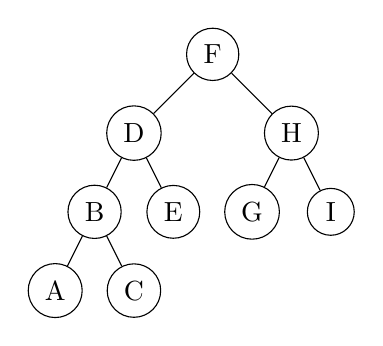
\begin{tikzpicture}[scale=.5]
            % \draw[step=1,color=gray!40] (-1,1) grid (8,9);
            \foreach \x/\y/\name in {1/4/B,3/4/E,4/8/F,5/4/G,7/4/I,2/6/D,6/6/H,2/2/C,0/2/A}{
                \node[black,draw,shape=circle,name=\name] at (\x,\y) {\name};
            }
            \foreach \from/\to in {F/D,F/H,D/B,D/E,B/C,H/G,H/I,B/A} {
                \draw (\from)--(\to) ;
            }
        \end{tikzpicture}
    \end{small}
\end{center}




 



\begin{lstlisting}[{style=v1,mathescape}]
typedef BiTree SOSTree;             //次优查找树采用二叉链表存储结构
int SecondOptimal(BiTree &T,ElemType R[],float sw[],int low ,int high){
    //由有序表R[low...high]及其累计权值表sw(sw[0]==1)递归构造次优查找数T
    i=low;min=abs(sw[high]-sw[low]);dw=sw[high]+sw[low-1];
    for(j=low+1;j<=high;++j){               //选择最小$\Delta P_i$值
        if(abs(dw-sw[j]-sw[j-1])<min){
            i=j;min=abs(dw-sw[j]-sw[j-1]);
        }
    }
    T=(BiTree)malloc(sizeof(BiTNode));
    T->data=R[i];                                   //生成节点
    if(i==low) T->lchild=NULL;                      //左子树空
    else SecondOptimal(T->lchild,R,sw,low,i-1);     //构造左子树   
    if(i==high) T->rchild=NULL;                     //右子树空
    else SecondOptimal(T->rchild,R,sw,i+1,high);    //构造右子树    
}

Status CreateSOSTree(SOSTree &T,SSTable ST){
    //有序表ST构造一棵次优查找树T,ST的数据元素含有权域weight
    if(ST.length==0) T=NULL;
    else{
        FindSW(sw,ST);      //按照有序表ST中各元素的weight域求累计权值表sw
        SecondOptimal(T,ST.elem,sw,1,ST.length);
    }
    return OK;
}

\end{lstlisting}



$$\begin{small}
    \ma{
        F_0=0,F_1=1\\    
        F_n&=F_{n-1}+F_{n-2} \q (n \geqslant 2)\\
        F_n-sF_{n-1}&=(1-s)(F_{n-1}+\frac{1}{1-s}F_{n-2}) \q (n \geqslant 2)\\
        &\meq{-s=\frac{1}{1-s}}{}(1-s)(F_{n-1}+sF_{n-2}) \q (n \geqslant 2)\\
        &=(1-s)^{n-1}(F_1+sF_0)  \\
        &=(1-s)^{n-1}\\
        F_n+k(1-s)^{n-1}&=sF_{n-1}+(1+k)(1-s)^{n-1}\\
        &=s[F_{n-1}+\frac{(1+k)}{s}(1-s)^{n-1}]\\
        &=s[F_{n-1}+\frac{(1+k)(1-s)}{s}(1-s)^{n-2}]\\
        &\meq{k=\frac{(1+k)(1-s)}{s}}{}s[F_{n-1}+k(1-s)^{n-2}]\\
        &=s^{n-1}[F_1+k(1-s)^0]\\
        &=s^{n-1}(1+k)\\
        F_n&=(1+k)s^{n-1}-k(1-s)^{n-1}\\
            &=\frac{1 \pm \sqrt{5}}{\pm 2\sqrt{5}}{(\frac{1\pm \sqrt{5}}{2})}^{n-1}- \frac{1 \mp \sqrt{5}}{\pm 2\sqrt{5}}{(\frac{1\mp \sqrt{5}}{2})}^{n-1}\\
            &=\frac{1}{\sqrt{5}}\mfc{\frac{1 \pm \sqrt{5}}{\pm 2 }{(\frac{1\pm \sqrt{5}}{2})}^{n-1}- \frac{1 \mp \sqrt{5}}{\pm 2 }{(\frac{1\mp \sqrt{5}}{2})}^{n-1}}\\
            &=\frac{1}{\sqrt{5}}\mfc{\frac{1 \pm \sqrt{5}}{\pm 2 }{(\frac{1\pm \sqrt{5}}{2})}^{n-1} \mp \frac{1 \mp \sqrt{5}}{ 2 }{(\frac{1\mp \sqrt{5}}{2})}^{n-1}}\\
            &=\fcz{
                \frac{1}{\sqrt{5}}\mfc{\frac{1 + \sqrt{5}}{+ 2 }{(\frac{1+ \sqrt{5}}{2})}^{n-1} - \frac{1 - \sqrt{5}}{ 2 }{(\frac{1- \sqrt{5}}{2})}^{n-1}}\\
                \frac{1}{\sqrt{5}}\mfc{\frac{1 - \sqrt{5}}{- 2 }{(\frac{1- \sqrt{5}}{2})}^{n-1} + \frac{1 + \sqrt{5}}{ 2 }{(\frac{1+ \sqrt{5}}{2})}^{n-1}}\\
            }\\
            &=\frac{1}{\sqrt{5}}\mfc{ {(\frac{1+ \sqrt{5}}{2})}^{n} -  {(\frac{1- \sqrt{5}}{2})}^{n}}\\
            &\approx  \frac{1}{\sqrt{5}} {(\frac{1+ \sqrt{5}}{2})}^{n} \\
            \fcz{
                -s=\frac{1}{1-s}\\
                k=\frac{(1+k)(1-s)}{s}
            }&\Rightarrow\fcz{
                -1-s+s^2=0\\
                ks=1-ks+k-s
            } \Rightarrow\fcz{
                s=\frac{1\pm \sqrt{5}}{2}\\
                (2s-1)k=1-s
            }\Rightarrow\fcz{
                s=\frac{1\pm \sqrt{5}}{2}\\
                1-s=\frac{1\mp \sqrt{5}}{2}\\
                k=\frac{1-s}{(2s-1)}=\frac{1 \mp \sqrt{5}}{\pm 2\sqrt{5}}\\
                1+k=\frac{1 \pm \sqrt{5}}{\pm 2\sqrt{5}}
            }

    }
\end{small}$$


 


\subsubsection{索引顺序表的查找}
 

$$
\ma{    
    ASL_{bs}&=L_b+L_w\\
    &=\frac{1}{b}\sum_{j=1}^bj+\frac{1}{s}\sum_{j=1}^sj\\
    &=\frac{1+b}{2}+\frac{1+s}{2}\\
    &=\frac{1}{2}(\frac{n}{s}+s)+1\\
    ASL_{bs}^{'}&\approxeq \log_2(\frac{n}{s}+1)-1+\frac{1+s}{2}\\
    &\approxeq\log_2(\frac{n}{s}+1)+\frac{s}{2}-\frac{1}{2}\\
    &\approxeq\log_2(\frac{n}{s}+1)+\frac{s}{2} 
}
$$







\subsection{动态查找表}

\subsubsection{二叉排序树和平衡二叉树}
\mb{二叉排序树及其查找过程}\p
\mb{二叉排序树}是空树或者具有性质$\ma{
    \mt{(1)非空左子树上所有节点小于根节点}\\
    \mt{(2)非空右子树上所有节点大于根节点}\\
    \mt{(3)左右子树分别为二叉排序树}\\
}$


\newpage

\mb{二叉排序树的插入和删除}\p
\begin{lstlisting}[style=v1]
    Status SearchBST(BiTree T,KeyType key,BiTree f,BiTree &p){
        //二叉排序树T中查找key
        //成功p指向节点,返回TRUE,失败p指向访问节点,返回FALSE
        //f指向双亲节点,初始值为NULL
        if(!T){p=f;return FALSE;}  //查找失败
        else if EQ(key,T->data.key){p=T;return TRUE;} //查找成功
        else if LT(key,T->data.key) return SearchBST(T->lchild,key,T,p);
        else  return SearchBST(T->rchild,key,T,p);
    }

    Status InsertBST(BiTree &T,ElemType e){
        //二叉排序树T中不存在key,插入e返回TRUE
        //否则返回FALSE
        if(!SearchBST(T,e.key,null,p)){
            s=(BiTree)malloc(sizeof (BiTNode));
            s->data=e;s->lchild=s->rchild=NULL;
            if(!p)T=s;
            else if(LT(e.key,P->data.key))p->lchild=s;
            else p->rchild=s;
            return TRUE;
        }
        else return FALSE;
    }


\end{lstlisting}

双亲节点$*f$删除节点$*p\ma{
    p_L,p_R\mt{均为空树,改双*f亲指针}\\
    p_L \, or \, p_R\mt{为空树,子树为双亲*f子树}\\
    p_L,p_R\mt{均不为空树,}\ma{
        (1)p_L\mt{为双亲*f左子树},p_r\mt{为}p_L\mt{最右}\\
        (2)p_L\mt{最右*s替代}*p,\mt{删除}*s\mt{重复操作}\\
    }
}$

% $$\ma{\sum_{j=1}^n -\ln n=\gamma\approx 0.577   \mt{(欧拉常数)}\\
% \frac{1}{2}<\sum_{j=1}^n -\ln n=\gamma <1 \\
% \sum_{j=2}^n -\ln n<0\\
% \sum_{j=2}^n<\ln n
% }$$

 \begin{lstlisting}[style=v1]
    Status DeleteBST(BiTree &T,KeyType key){
        //若二叉树T中存在key,删除该节点
        //并返回TRUE,否则返回FALSE
        if(!T) return FALSE;            //不存在key
        else{
            if(EQ(key,T->data.key)) return Delete(T);  //找到key
            else if(LT(k,T->data.key)) return DeleteBST(T->lchild,key);
            else return DeleteBST(T->rchild,key); 
        }
    }

    Status Delete(BiTree &p){
        //从二叉树删除节点p,重接左子树或右子树
        if(!p->rchild){q=p;p=p->lchild;free(q);}
        else if(!p->lchild){q=p;p=p->rchild;free(q);}
        else{
            q=p;s=p->lchild;                    //左转
            while(s->rchild){q=s;s=s->rchild;}  //右转到尽头,
            p->data=s->data;                    //s指向p前驱,q指向s双亲
            if(q!=p)q->rchild=s->lchild;  //重接q右子树  
            else q->lchild=s->lchild;     //重接q右子树(左单支)
            free(s);
        }
        return TRUE;
    }
 \end{lstlisting}

\mb{二叉排序树的查找分析}\p




$$
\begin{small}  
    \ma{
    \mf{\frac{a_1+a_2+\cdots+a_n}{n}}^n\geqslant a_1a_2\dots a_n\\
    e=\lim_{n \rightarrow \infty}(1+\frac{1}{n})^n \approx 2.76 \mt{(自然常數)}\\
    s_n=(1+\frac{1}{n})^n=(\frac{1+n}{n})^n\cdot 1\leqslant\mf{\frac{\frac{n+1}{n}+\dots+\frac{n+1}{n}+1}{n+1}}^{n+1}=(\frac{n+2}{n+1})^{n+1}=s_{n+1},\mt{單增}
    \q n\geqslant 1\\
    t_n=\mf{1+\frac{1}{n}}^{n+1}=\mf{\frac{n+1}{n}}^{n+1},\mt{單減} \q n\geqslant 1\\
    \frac{1}{t_n}=\mf{\frac{n}{n+1}}^{n+1}=\mf{\frac{n}{n+1}}^{n+1}\cdot 1 \leqslant \mf{\frac{\frac{n}{n+1}+\dots +\frac{n}{n+1} +1}{n+2}}^{n+2}=\mf{\frac{n+1}{n+2}}^{n+2}=\frac{1}{t_{n+1}}
    ,t_n\geqslant t_{n+1}\\
    2=s_1<s_n<t_n<t_1=4\\
    (1+\frac{1}{n})^n <s_{max}=e<t_{min}< (1+\frac{1}{n})^{n+1},
    % n\ln (1+\frac{1}{n})<1< (n+1)\ln (1+\frac{1}{n})\\
    n\ln (\frac{n+1}{n})<1< (n+1)\ln (\frac{n+1}{n})\\
    \frac{1}{n+1}<\ln (\frac{n+1}{n})<\frac{1}{n}
    }
 \end{small}
$$

$$
\begin{small}
    \ma{
    \gamma_n=1+\frac{1}{2}+\frac{1}{3}+\dots+\frac{1}{n}-\ln n\\
    >\ln (\frac{2}{1})+\ln (\frac{3}{2})+\ln (\frac{4}{3})+\dots+\ln (\frac{n+1}{n})-\ln n\\
    >\ln(n+1)-\ln n>0,\mt{正项}\\
    \gamma_{n+1}-\gamma_n=\frac{1}{n+1}-\ln(n+1)+\ln n=\frac{1}{n+1}-\ln(\frac{n+1}{n})<0,\gamma_{n+1}<\gamma_n,\mt{单减}\\
    0<\gamma_n<1\\
    k=\sum_{j=1}^n \frac{1}{j}\\
    \int_1^n \frac{1}{x}dx=\ln n<1+\frac{1}{2}+\frac{1}{3}+\dots+\frac{1}{n-1}=k+\frac{1}{n}\\
    \int_1^n \frac{1}{x}dx=\ln n>\frac{1}{2}+\frac{1}{3}+\frac{1}{3}+\dots+\frac{1}{n}=k-1\\
    \int_1^n \frac{1}{x}dx=\ln n<\frac{1}{2}(1+\frac{1}{2})+\frac{1}{2}(\frac{1}{2}+\frac{1}{3})+\frac{1}{2}(\frac{1}{3}+\frac{1}{4})+\dots+\frac{1}{2}(\frac{1}{n-1}+\frac{1}{n})=k-\frac{1}{2n}-\frac{1}{2}\\
    
    \frac{1}{2}<\frac{1}{2}+\frac{1}{2n}<(k-\ln n)=\gamma_n<1\\
    k -\ln n=\gamma\approx 0.577   \mt{(欧拉常数)}\\
    % \frac{1}{2}<\sum_{j=1}^n\frac{1}{j} -\ln n=\gamma <1 \\
    % \sum_{j=2}^n\frac{1}{j} -\ln n<0\\
    \sum_{j=2}^n\frac{1}{j}=k-1=\ln n+\gamma-1<\ln n\\
    }
\end{small}
$$


$$\ma{
    P(n,i)=\frac{1}{n}[1+i\cdot (P(i)+1)+(n-i-1)\cdot (P(n-i-1)+1)]\\
    P(n)=\frac{1}{n}\sum_{i=0}^{n-1}P(n,i)\\
    =\frac{1}{n} \sum_{i=0}^{n-1}\frac{1}{n} [1+i\cdot (P(i)+1)+(n-i-1)\cdot (P(n-i-1)+1)]\\
    =\frac{1}{n^2} \sum_{i=0}^{n-1}[ i\cdot P(i)+i+1+(n-i-1)\cdot P(n-i-1)+n-i-1]\\
    =\frac{1}{n^2} \sum_{i=0}^{n-1}[ i\cdot P(i) +(n-i-1)\cdot P(n-i-1)+n ]\\
    =1+\frac{1}{n^2} \sum_{i=0}^{n-1}[ i\cdot P(i) +(n-i-1)\cdot P(n-i-1) ]\\
    =1+\frac{1}{n^2} [0\cdot P(0)+(n-1)\cdot P(n-1)+  1\cdot P(1)+(n-2)\cdot P(n-2)+\dots + (n-1)\cdot P(n-1) +0\cdot P(0) ]\\
    =1+\frac{2}{n^2} \sum_{i=0}^{n-1}i\cdot P(i)\\
    k_n=\sum_{i=0}^{n-1}i\cdot P(i),k_{n-1}=\sum_{i=0}^{n-2}i\cdot P(i)\\
    k_n=k_{n-1}+(n-1)P(n-1)\\
    P(n)=1+\frac{2}{n^2}k_n\\
    P(n-1)=1+\frac{2}{(n-1)^2}k_{n-1}\\
    \frac{n^2}{2}\mf{P(n)-1}=\frac{(n-1)^2}{2}\mf{P(n-1)-1}+(n-1)P(n-1)\\
    P(n)= \frac{n^2-1}{n^2}P(n-1)+ \frac{2n-1}{n^2},P(1)=1,P(0)=0\\
    \frac{n}{n+1}P(n)=\frac{n-1}{n}P(n-1)+\frac{2n-1}{n(n+1)}\\
    s_n=\frac{n}{n+1}P(n),\delta_n=\frac{2n-1}{n(n+1)}\\
    s_n=s_{n-1}+\delta_n\\
    s_{n-1}=s_{n-1}+\delta_{n-1}\\
    \dots\\
    s_2=s_1+\delta_2\\
    s_1=s_0+\delta_1\\
    s_n=\sum_{j=1}^{n} \delta_j=\sum_{j=1}^{n} \frac{2j-1}{j(j+1)}=\sum_{j=1}^{n} (2j-1)(\frac{1}{j}-\frac{1}{j+1})\\
    =\sum_{j=1}^{n} \frac{2j-1}{j} -\frac{2j-1}{j+1}\\
    =\sum_{j=1}^{n} \frac{2j-1}{j} -\frac{2j+2-3}{j+1}\\
    =\sum_{j=1}^{n} \frac{-1}{j} +\sum_{j=1}^{n} \frac{3}{j+1} \\
    =\sum_{j=1}^{n} \frac{-1}{j} +\sum_{j=1}^{n} \frac{1+2}{j+1} \\
    =\sum_{j=1}^{n} (\frac{-1}{j}+\frac{1}{j+1}) +\sum_{j=1}^{n} \frac{2}{j+1}\\
    =-\frac{n}{n+1}+\sum_{j=1}^{n} \frac{2}{j+1}\\
    P(n)=\frac{n+1}{n}s_n=-1+2\frac{n+1}{n} \sum_{j=1}^{n} \frac{1}{j+1}=-1+2\frac{n+1}{n} (\frac{1}{2} +\frac{1}{3}+\dots+\frac{1}{n+1}  )\\
    =2\frac{n+1}{n} (\frac{1}{2} +\frac{1}{3}+\dots+\frac{1}{n}  ) +\frac{2}{n}-1\\
    =2\frac{n+1}{n} (k-1)+\frac{2}{n}-1=2\frac{n+1}{n} (\ln n +\gamma-1)+\frac{2}{n}-1 \leqslant 2\frac{n+1}{n} \ln n 

}$$




\newpage


\mb{平衡二叉树} 是空树或者具有性质 $\ma{
    (1) \mt{左右子树都是平衡二叉树}\\
    (2) \mt{左右子树高度差绝对值小于1}\\
}$

\mb{平衡因子}左子树高度减右子树高度

\mb{失衡调整}  $\ma{
    (1) \mt{单向右旋}\\
    (2) \mt{单向左旋}\\
    (3) \mt{双向旋转(先左后右)}\\
    (4) \mt{双向旋转(先右后左)}
}$   \mb{插入e算法描述} $\ma{
    (1) \mt{空树,e为根节点}\\
    (2) \mt{e等于根节点,不插入}\\
    (3) \mt{e小于根节点,左子树无e,插入左子树}\\
    \q \ma{
        \mt{根节点平衡因子=-1,改为0,树深度+0}\\
        \mt{根节点平衡因子=0,改为1,树深度+1}\\
        \mt{根节点平衡因子=1}\\
        \q \ma{
            \mt{左子树根节点平衡因子=1,单向右旋}\\
            \mt{左子树根节点平衡因子=-1,先左后右}\\
        }
    }\\
    (4) \mt{e大于根节点,右子树无e,插入右子树}\\
    \q \ma{
        \mt{根节点平衡因子=1,改为0,树深度+0}\\
        \mt{根节点平衡因子=0,改为1,树深度+1}\\
        \mt{根节点平衡因子=-1}\\
        \q \ma{
            \mt{右子树根节点平衡因子=-1,单向左旋}\\
            \mt{右子树根节点平衡因子=1,先右后左}\\
        }
    }\\
}$ 

\begin{lstlisting}[style=v1]
    #define LH +1;
    #define EH 0;
    #define RH -1;

    typedef struct BSTNode{
    int bf;                             //节点平衡因子
    struct BSTNode * lchild ,*rchild;   //左右孩子指针
    }BSTNode,*BSTree;

    void R_Rotate(BSTree &p){
        //对以*p为根的二叉排序树作右旋处理,处理后p指向新的根节点,即左子树根节点
        lc=p->lchild;               //lc指向*p的左子树的根节点
        p->lchild=lc->rchild;       //lc的右子树挂接为*p的左子树    
        lc->rchild=p;p=lc;          //p指向新的根节点
    }

    void L_Rotate(BSTree &p){
        //对以*p为根的二叉排序树作左旋处理,处理后p指向新的根节点,即右子树根节点
        rc=p->rchild;               //rc指向*p的右子树的根节点
        p->rchild=rc->lchild;       //rc的左子树挂接为*p的右子树    
        rc->lchild=p;p=rc;          //p指向新的根节点
    }

    void LeftBalance(BSTree &T){
        //对平衡二叉树T作左平衡处理,结束时T指向新的根点
        lc=T->lchild;
        switch(lc->bf){
            case LH:
                T->bf=lc-bf=EH; R_Rotate(T);break;
            case RH:
                rd=lc->rchild;
                switch(rd->bf){
                    case LH:T->bf=RH;lc->bf=Eh;break;
                    case EH:T->bf=lc->bf=EH;break;
                    case RH:T->bf=EH;lc->bf=LH;break;
                }
                rd->bf=EH;
                L_Rotate(T->rchild);
                R_Rotate(T);
        }
    }



\end{lstlisting}

\newpage


\begin{lstlisting}[style=v1]
    Status InsertAVL(BSTree &T,ElemType e,Boolean &taller){
        //平衡二叉树T不存在e,插入返回1,否则返回0
        //若插入失衡,则平衡处理,taller反映长高与否

        if(!T){
            T=(BSTree) malloc(sizeof(BSTNode));T->data=e;
            T->lchild=T->rchild=NULL;T->bf=EH;taller=TRUE;
        }
        else{
            if(EQ(e.key,T->data.key)){taller=FALSE;return 0;}
            if(LT(e.key,T->data.key)){
                if(!InsertAVL(T->lchild,e,taller)) return 0;
                if(taller) switch(T->bf){
                    case LH:
                        LeftBalance(T);taller=FALSE;break;
                    case EH:
                        T->bf=LH;taller=TRUE;break;
                    case RH:
                        T->bf=EH;taller=FALSE;break;
                }
            }
            else{
                if(!InsertAVL(T->rchild,e,taller)) return 0;
                if(taller) switch(T->bf){
                    case LH:
                        T->bf=EH;taller=FALSE;break;
                    case EH:
                        T->bf=RH;taller=TRUE;break;
                    case RH:
                        RightBalance(T);taller=FALSE;break;
                }
            }
        }
        return 1;
    }
\end{lstlisting}





\mb{平衡二叉树查找的分析}\p
比较次数不超过树的深度

$N_h$深度为h的平衡二叉树的最少节点数

% $N_0=0,N_1=1,N_2=2,N_h=N_{h-1}+N_{h-2}+1$

$
\ma{
% N_0=0,N_1=1,N_2=2,N_h=N_{h-1}+N_{h-2}+1\\
N_{n+1}+1=N_n+1+N_{n-1}+1,N_0=0,N_1=1,N_2=2\\
b_{n+1}=b_n+b_{n-1},b_0=1,b_1=2,b_2=3\\
b_{n+1}-s b_n=(1-s)(b_n-s b_{n-1})=(1-s)^n(b_1-s b_0)=(2-s)(1-s)^n\\
    \q  (s-1)s=1, s_1=\frac{1+\sqrt{5}}{2},s_2=\frac{12\sqrt{5}}{2}\\
b_{n+1}-s_1 b_n=(2-s_1)(1-s_1)^n\\
b_{n+1}-s_2 b_n=(2-s_2)(1-s_2)^n\\
-(s_2-s_1)b_n=(2-s_2)(1-s_2)^n-(2-s_1)(1-s_1)^n\\
% =(1-s_2)(1-s_2)^n-(1-s_1)(1-s_1)^n+ (1-s_2)^n-(1-s_1)^n \\
% = (1-s_2)^{n+1}- (1-s_1)^{n+1}+ (1-s_2)^n-(1-s_1)^n \\
s_2-s_1=-\sqrt{5},2-s_2=\frac{3+\sqrt{5}}{2},2-s_1=\frac{3-\sqrt{5}}{2},1-s_2=\frac{1+\sqrt{5}}{2},1-s_1=\frac{1-\sqrt{5}}{2}\\
b_n=\frac{(2-s_2)}{-(s_2-s_1)}(1-s_2)^n-\frac{(2-s_1)}{-(s_2-s_1)}(1-s_1)^n\\
b_n=\frac{1}{\sqrt{5}}\mfc{(1+\frac{1+\sqrt{5}}{2})(\frac{1+\sqrt{5}}{2})^n - (1+\frac{1-\sqrt{5}}{2})(\frac{1-\sqrt{5}}{2})^n }=F_n+F_{n+1}\\
N_n=b_n-1=F_n+F_{n+1}-1=F_{n+2}-1\\
F_h \approx \frac{1}{\sqrt{5}}\mf{\frac{1+\sqrt{5}}{2}}^h=c(\varphi)^h\\
N_h=c(\varphi)^{h+2}-1\\
\log (\frac{N_h+1}{c})=(h+2)\log \varphi\\
\frac{\log (\frac{N_h+1}{c})}{\log \varphi}-2=\log _\varphi (\frac{N_h+1}{c}) -2=h
}
$

 先排序,再构造次优查找树,生成树是二叉排序树



\newpage

\subsubsection{B-树和B+树}

\mb{B-树及其查找}\p

\mb{B-树}是平衡的多路查找树,

m阶\mb{B-树}是空树或具有性质$\ma{
    (1)\mt{每个节点至多有m棵子树}\\
    (2)\mt{若根节点不是叶子节点,则至少有两棵子树}\\
    (3)\mt{除根结点之外的所有非终端节点,至少包含} \lceil \frac{m}{2} \rceil\mt{棵子树}\\
    (4)\mt{所有的非终端节点,包含信息}\\
        \q (n,A_0,k_1,A_1,K_2,\dots,K_n,A_n),
        K_i\mt{为关键字},A_i\mt{指向根节点的指针}\\
        \q A_{i-1}\mt{指向子树的所有节点小于} K_i,
        A_{i+1}\mt{指向子树的所有节点大于} K_i\\
        \q \mt{关键字个数}n ,\lceil \frac{m}{2} \rceil -1  \leqslant n\leqslant m-1\\
    (5)\mt{所有的叶子节点都出现在同一层次上,且不带信息}\\
}$

% \newpage

\begin{lstlisting}[style=v1]
    #define m 3                     //B-树的阶
    typedef struct BTNode{
        int keynum;                 //关键字个数,即节点大小
        struct BTNode * parent;     //双亲结点   
        KeyType key[m+1];           //关键字向量,0号单元未用
        struct BTNode * ptr[m+1];   //子树指针向量
        Record *recptr[m+1];        //记录指针向量,0号单元未用
    }BTNode,*BTree;

    typedef struct{
        BTNode *pt;         //指向找到的节点
        int i;              //在节点中的关键字号    
        int tag;            //1成功,0失败
    }Result;                //B-树查找结果类型


    Result SearchBTree(BTree T,KeyType K){
        //在m阶B-树T上查找K,返回(pt,i,tag)
        //成功返回位置,失败插入返回插入位置
        p=T;q=NULL;found=FALSE;i=0;     //初始化,p指向待查节点,q指向p的双亲节点
        while(p && !found){
            i=Search(p,k);              //在p->key [1...keynum]中查找
            if(i>0 && p->key[i]==k) found =TRUE;    //查到关键字
            else{q=p;p=p->ptr[i];}
        }
        if(found) return (p,i,1);
        else return (q,i,0);
    }
\end{lstlisting}

\mb{B-树查找分析}\p

磁盘节点,内存顺序

$1,2,2\mfd{\frac{m}{2}},2\mfd{\frac{m}{2}}^2,\dots,2\mfd{\frac{m}{2}}^{n-2},\dots$

N关键字B-树,深度l+1(叶子算深度),N+1叶子节点

$\ma{N+1\geqslant 2\mfd{\frac{m}{2}}^{l+1-2}\\
    \log_{\mfd{\frac{m}{2}}} (N+1) \geqslant \log_{\mfd{\frac{m}{2}}} 2 +l-1\\
    \log_{\mfd{\frac{m}{2}}} (\frac{N+1}{2}) +1 \geqslant  l
}$

\mb{B-树插入和删除}\p


最底层非终端节点添加,添加后关键字个数不超过m-1完成,超过分裂

\mb{节点分裂}$*p$节点含m-1关键字,插入后节点信息$(m,A_0,K_1,A_1,K_2,A_2,\dots,K_m,A_m)$

$\q *p_1,(\mfd{\frac{m}{2}}-1,A_0,K_1,A_1,K_2,A_2,\dots,K_{\mfd{\frac{m}{2}}-1},A_{\mfd{\frac{m}{2}}-1}) $

$\q *p_2,(m-\mfd{\frac{m}{2}},A_{\mfd{\frac{m}{2}}},K_{\mfd{\frac{m}{2}}+1},A_{\mfd{\frac{m}{2}}+1},K_{\mfd{\frac{m}{2}}+2},A_{\mfd{\frac{m}{2}}+2},\dots,K_m,A_m) $

$\q key,(K_{\mfd{\frac{m}{2}}},*p_2) $ 合并到双亲


\newpage

\begin{lstlisting}[style=v1]
    Status InsertBtree(BTree &T ,KeyType T,BTree q ,int i){
        //m阶B-树,*q的key[i],key[i+1]之间插入关键字k
        //插入后节点过大则分裂
        x=k;ap=NULL;finished=FALSE;
        while(q && !finished){
            Insert(q,i,x,ap);       //将x,ap分别插入q->key[i+1],q->ptr[i+1],
            if(q->keynum<m) finished=TRUE;      //插入完成
            else{                               //分裂节点*q
                s=m/2+1;splite(q,s,ap);x=q->key[s];   
                //移动相应元素q->key[s+1..m], q->ptr[s..m]q->recptr[s+1..m]到新节点*ap
                q=q->parent;
                if(q) i=Search(q,x);
            }
        }
        if(!finished)             //T是空树或者节点已分裂为节点*p,*ap      
            NewRoot(T,q,x,ap);    //生成含信息(T,x,ap)的新的根节点*T,原T和ap为子树指针 
        return OK;
    }
   
\end{lstlisting}

最底层非终端节点删除,删除后关键字个数不小于$\mfd{\frac{m}{2}}$完成,小于合并

非终端节点$K_i$用指针$A_i$子树最小关键字Y替代$K_i$再删除Y

非终端删除情况(关键字个数)$\ma{
    (1) \mt{所在节点大于等于} \mfd{\frac{m}{2}}\\
    (2) \mt{所在节点等于} \mfd{\frac{m}{2}}-1 ,\mt{存在兄弟节点大于} \mfd{\frac{m}{2}}-1,\mt{双亲借兄弟,靠近给自己}\\
    (3) \mt{所在节点等于} \mfd{\frac{m}{2}}-1 ,\mt{兄弟节点都等于} \mfd{\frac{m}{2}}-1,\mt{毁灭自己,留给兄弟}
}$

\subsubsection{键树}

\mb{键树}又称数字查找树,度大于2的树。元素是组成关键字的符号。关键字是数值,单词。

\mb{键树}是有序树,结束符$\$$小于任何字符

\mb{键树存储结构}\q

    (1)孩子兄弟链表,分支节点 $(symbol,first,next)$,叶子节点$infoptr$域,双链树

\begin{lstlisting}[style=v1]
    #define MAXKEYLEN 16        //关键字最大长度
    typedef struct{             
        char ch[MAXKEYLEN];     //关键字
        int num;                //关键字长度
    }KeysType;                  //关键字类型

    typedef enum{LEAF,BRANCH} NodeKind;     //节点种类:{叶子,分支}
    typedef struct DLTNode{
        char symbol;
        struct DLTNode *next;              //指向兄弟节点的指针 
        NodeKind kind;
        union{
            Record *infoptr;              // 叶子节点的记录指针
            struct DLTNode *first         // 分支节点的孩子链指针 
        }
    }DLTNode,*DLTree;                      //双链树的类型 

    Record * SearchDLTree(DLTree T,KeysType K){
        //在非空双链树T中查找K,存在返回记录指针,失败返回空指针
        p=-T->first;i=0;
        while(p&& i<k.num){
            while(p&& p->symbol !=K.ch[i]) p=p->next;       //查找第i
            if(p&& i<K.num-1) p=p->first;                   //准备查找下一位
            ++i;
        }
        if(!p) return NULL;                                 //查找成功
        else return p->infoptr;                             //查找失败   
    }



\end{lstlisting}

键树节点最大度d,深度h,双链树平均查找长度 $\frac{h}{2}(1+d)$

插入删除节点,等于在树中某个节点插入删除子树

(2)多重链表,单支树压缩为叶子节点,

\begin{lstlisting}[style=v1]
    typedef struct TrieNode{
        NodeKind kind;
        union{
            struct{KeysType k;Record * infoptr;} lf;   //叶子节点
            struct{TrieNode *ptr[27]; int num;} bh;    //分支节点
        }
    }TrieNode,*TrieTree;

    Record * SearchTrie(TrieTree T,KeysType k){
        //在键树T中查找关键字等于K的记录
        for(p=T,i=0;                                    //对k的每个字符逐个查找
            p&& p->kind==BRANCH && i<K.num;             //*p为分支节点
            p=p->bh.ptr[ord(K.ch[i])],++i);              //ord 求字符在字母表中序号,$为0   
        if(p=&& p->kind==LEAF&& p->lf.k==k) return p->lf.infoptr;  //查找成功
        else return NULL;
    }


\end{lstlisting}   

多重链表键树分割,无查找分析

\subsection{哈希表}

\subsubsection{哈希表}


$\mt{關鍵字}k,\mt{象} f(k),\mt{對應關係}f,\mb{哈希函數}$

$\ma{\
    (1) mt{哈希函數是映像}\\
    (2) \mt{不同關鍵字同象}\mb{衝突}\\
    (3) \mt{關鍵字象做位置,以哈希函數,衝突處理辦法映射關鍵字到連續地址} \mb{哈希表}\\
    (4) \mt{映射過程}\mb{散列},\mt{存儲位置}\mb{哈希地址或散列地址}
}$
 

\subsubsection{哈希函數構造方法}

關鍵字映射到地址等概率\mb{均勻哈希函數}

$\ma{
    (1) \mt{直接定地址} H(key)=a \cdot key +b\\
    (2) \mt{數字分析}\\
    (3) \mt{平方取中}\\
    (4) \mt{折疊法,(移位折疊,間界折疊)}\\
    (5) \mt{除留餘數}  H(key)=key MOD p\mt{(質數,不小於20質因數的合數)}, p \leqslant m\mt{(表長)}\\
    (6) \mt{隨機數}   H(key)=random(key)  
}$

\subsubsection{衝突處理方法}

地址序列

$\ma{
    (1) \mt{開放定址法} H_i=(H(key)+d_i) \, MOD\,  m \q i=1,2,\dots,k (k\leqslant m)\\
    \q \ma{
        d_i \mt{取法} &(1) d_i=1,2,3,\cdots,m-1  \mt{,線性探測再散列}\\
        &(2) d_i=1^2,-1^2,2^2,-2^2,3^2,\cdots,\pm k^2  \mt{,二次探測再散列}\\
        &(3) d_i=\mt{偽隨機數列,}\mt{隨機探測再散列}
    }\\
    \q \mt{處理同義詞衝突產生非同義詞衝突,}\mb{二次聚集}\\
    \q \mt{線性能填滿;平方形如}m=4j+3\mt{的素數能填滿;隨機數列}\\
    (2) \mt{再哈希法} H_i=RH_i(key) \q i=1,2,\dots,k\\
    (3) \mt{鏈地址法} Chain ChainHash[i]\\
    (4) \mt{公共溢出區} HashTable[0..m-1],OverTable[0..v]
}$


\newpage
\subsubsection{哈希表的查找及其分析}

有記錄,且記錄等於關鍵字則查找成功

\begin{lstlisting}[style=v1]
    \\---開放地址哈希表的存儲結構
    int Hashsize[]={997,...};       //哈希容量遞增表,一個合適的素數序列
    typedef struct{
        ElemType * elem;            //數據元素存儲基址,動態分配數組
        int count;                  //當前數據元素個數    
        int sizeindex;              //Hashsize[sizeindex]為當前容量
    }HashTable;

    #define SUCCESS 1
    #define UNSUCCESS 0
    #define DUPLICATE -1

    Status SearchHash(HashTable H,KeyType k,int &p,int &c){
        //在開放地址哈希表中查找關鍵碼為k的元素
        //成功p指向节点,返回SUCCESS。失敗p指向插入位置,返回UNSUCCESS
        //c用作衝突計數,初始值0,供建表插入時參考
        p=Hash(k);
        while(H.elem[p].key !=NULLKEY &&        //有記錄
            !EQ(k,H.elem[p].key))               //關鍵字不等
            colision(p,++c);                    //求得下一探查地址
        if(EQ(k,H.elem[p].key)) return SUCCESS; //成功,p返回位置
        else return UNSUCCESS;                  //失敗,p返回插入位置
    }
 
    Status InsertHash(HashTable &H,ElemType e){
        //查找不成功插入e到H,返回OK
        //衝突次數過大則重建哈希表
        c=0;
        if(SearchHash(H,e.key,c)) return DUPLICATE;     //表中有e
        else if(c<Hashsize[H.sizeindex]/2){             //衝突次數未達到上限   
            H.elem[p]=e;++H.count;return OK;            //插入e
        }
        else{
            RecreateHashTable(H);return UNSUCCESS;      //重建哈希表
        }
    }
 
\end{lstlisting}


哈希表裝填因子  $\alpha=\frac{\mt{表中填入記錄數}}{\mt{哈希表長度}}$


$\ma{
    \mt{成功時平均查找長度}
    &S_{nl} \approx \frac{1}{2}\mf{1+\frac{1}{1-\alpha}} \mt{線性探測再散列}\\
    &S_{nr} \approx -\frac{1}{\alpha} \ln \mf{1 -\alpha} \mt{偽隨機探測,二次探測,再哈希}\\
    &S_{nc} \approx 1+\frac{\alpha}{2} \mt{鏈地址法}
}$

$\ma{
    \mt{失敗時平均查找長度}
    &U_{nl} \approx  \frac{1}{2}\mf{1+\frac{1}{(1-\alpha)^2}} \mt{線性探測再散列} \\
    &U_{nr} \approx  \frac{1}{1-\alpha} \mt{偽隨機探測,二次探測,再哈希}\\
    &U_{nc} \approx  \alpha + e^{-\alpha} \mt{鏈地址法}
}$




\newpage
\section{内部排序}


\subsection{概述}

\begin{lstlisting}[style=v1]
 #define MAXSIZE 20
 typedef int KeyType;
 typedef struct{
    KeyType key;
    InfoType ontherinfo;
 }RedType;
typedef struct{
    RedType r[MAXSIZE+1];
    int length;
}Sqlist;
\end{lstlisting}


\subsection{插入排序}
\subsubsection{直接插入}

\begin{lstlisting}[style=v1]
    void InsertSort(Sqlist &L){
        //对顺序表做直接插入排序
        for(i=2;i<=L.length;i++){
            if(LT(L.r[i].key,L.r[i-1].key)){ //"<",需将L.r[i]插入有序子表
                L.r[0]=L.r[i];               //复制为哨兵
                L.r[i]=L.r[i-1];
                for(j=i-2;LT(L.r[0].key,L.r[j].key);--j)
                    L.r[j+1]=L.r[j];         //记录后移  
                L.r[j+1]=L.r[0];             //插入正确位置
                printf("vine");
            }
        }
    }//InsertSort
\end{lstlisting}

\subsubsection{其他插入}

\mb{折半插入}
\begin{lstlisting}[style=v1]
    void BInsertSort(Sqlist &L){
        //对顺序表做折半插入排序
        for(i=2;i<=L.length;i++){
            L.r[0]=L.r[i];                  //将L.r[i]暂存到L.r[0]
            low=1,high=i-1;
            while(low<=high){               //在L.r[low...high]中折半查找有序插入位置
                m=(low+high)/2;             //折半
                if(LT(L.r[0].key,L.r[m].key)) high=m-1; //插入点在高
                else low =m+1;                          //插入点在低   
            }
            for(j=i-1;j>=high+1;--j) L.r[j+1]=L.r[j];   //记录后移
            L.r[high+1]=L.r[0];                         //插入
        }
    }//BInsertSort
\end{lstlisting}\p
\mb{二路插入}\p
\mb{表插入}\p

\newpage
\mb{希尔排序}

\begin{lstlisting}[style=v1]

    void ShellInsort(Sqlist &L,int dk){
        //对顺序表做希尔插入排序
        //1.位置增量dk
        //2.L.r[0]是暂存不是哨兵,j<=0时插入位置已找到
        for(i=dk+1;i<=L.length;i++){
            if(LT(L.r[i].key,L.r[i-dk].key)){ //"<",需将L.r[i]插入有序子表
                L.r[0]=L.r[i];               //暂存L.r[0]
                for(j=i-dk;j>0 && LT(L.r[0].key,L.r[j].key);j-=dk)
                    L.r[j+dk]=L.r[j];         //记录后移,查找插入位置
                L.r[j+dk]=L.r[0];             //插入正确位置
            }
        }
    }//ShellInsort

    void ShellSort(Sqlist &L,int dk[],int t){
        //按增量序列 dk[0...t-1]对顺序表做希尔插入排序
        for(k=0;k<t;k++){
            ShellInsort(L,dk[k]);     //一趟增量为dk[k]的插入排序
        }
    }//ShellSort


\end{lstlisting}

 

\subsection{快速}
\subsubsection{起泡排序}

\begin{lstlisting}[style=v1]
    void BubbleSort(int a[],int n){
        for(i=n-1,change=TRUE;i>=1 && change;--i){
            change=FALSE;
            for(j=0;j<i,j++){
                if(a[j]>a[i]){SWAP(a[j],a[i]);change=TRUE;}
            }
        }
    }
\end{lstlisting}



\subsubsection{快速排序}
 
\begin{lstlisting}[style=v1]
    void Partition(Sqlist &L,int low,int high){
        //交换顺序表L中子序列L.r[low...high]的记录,枢轴记录到位,返回位置此时
        //在枢轴前(后)记录不大于(不小于)它
        L.r[0]=L.r[low];        //第一个记录做枢轴
        pivotkey=L.r[low].key;  //枢轴记录关键字
        while(low<high){        //从表的两端交替向中间扫描
            while(low<high && L.r[high].key>=pivotkey) --high;
            L.r[low]=L.r[high];  //小的左移
            while(low<high && L.r[low]<=pivotkey) ++low;
            L.r[high]=L.r[low];  //大的右移   
        }
        L.r[low]=L.r[0];         //枢轴到位  
        return low;              //返回枢轴位置  
    }

    void QSort(Sqlist &L,int low,int high){
        //对顺序表L中子序列L.r[low...high]作快速排序
        if(low<high){                       //长度大于1
            pivotkey=Partition(L,low,high); //将L.r[low...high]一分为二
            QSort(L,low,pivotkey-1);        //低子表递归
            QSort(L,pivotkey+1,high);       //高子表递归
        }
    }

    void QuickSort(Sqlist &L){
        //对顺序表L作快速排序
        QSort(L,1,L.length)
    }

\end{lstlisting}
 
\subsection{选择排序}
 
\subsubsection{简单选择排序}

\begin{lstlisting}[style=v1]
    void SelectSort(Sqlist &L ){
        for(i=1;i<L.length;i++){        //选择第i小的记录,并交换到位
            j=SelectMinKey(L,i);        //在L.r[i...L.length]中选择key最小的记录
            if(i!=j) SWAP(L.r[i],L.r[j]) //与第i个记录交换
        }
    }
\end{lstlisting}
\subsubsection{树形排序}

% \newpage
\subsubsection{堆排序}


\begin{lstlisting}[style=v1]
    void HeapAdjust(HeapType &H,int s ,int m ){
        //已知H.r[s...m]中记录除H.r[s]外均满足堆的定义
        //调整H.r[s]使得H.r[s...m]称为大顶堆
        rc=H.r[s];
        for(j=2*s;j<=m;j*=2){    //沿key较大的孩子节点向下筛选
            if(j<m && LT(H.r[j].key,H.r[j+1].key)) ++j; //j为key较大的记录的下标
            if(!LT(rc.key,H.r[j].key)) break;           //rc插入s    
            H.r[s]=H.r[j];s=j;                           //插入   
        }
        H.r[s]=rc;
    }
 
    void HeapSort(HeapType &H ){
        for(i=H.length/2;;i>0;--i)            //把H.r[1...H.length]建成大顶堆          
            HeapAdjust(H,i,H.length);           
        for(i=H.length;i>1;--i){               //堆顶记录和未经排序子序列H.r[1...i]中最后一个记录交换 
            SWAP(H.r[1],H.r[i]);                //将[1...i-1]建成大顶堆
            HeapAdjust(H,1,i-1); 
        }
    }
 
\end{lstlisting}





\subsection{归并排序}

\begin{lstlisting}[style=v1]
    void Merge(RcdType SR[],RcdType & TR[],int i,int m,int n ){
        //将有序的SR[i...m],SR[m+1,n]归并为有序的TR[i...n]
        for(j=m+1,k=i;i<=m && j<=n;++k){  //将SR中记录从小到大并入TR
            if(LQ(SR[i].key,SR[j].key))  TR[k]=SR[i++];
            else TR[k]=SR[j++];
        }
        if(i<=m) TR[K...n]=SR[i...m];       //将剩余的SR[i...m]复制到TR[K...n]
        if(j<n)  TR[k...n]=SR[j...n];       //将剩余的SR[j...n]复制到TR[K...n]
    }

    void Msort(RcdType SR[],RcdType & TR1[],int s,int t){
        //将SR[s...t]归并为TR1[s...t]
        if(s==t) TR1[s]=SR[s];
        else{
            m=(s+t)/2;           //将SR[s...t]平分为SR[s...m],SR[m+1...t]
            Msort(SR,TR2,s,m);   //递归SR[s...m] 为有序 TR2[s...m]  
            Msort(SR,TR2,m+1,t);  //递归SR[m+1...t]为有序 TR2[m+1...t] 
            Merge[TR2,TR1,s,m.t]; //将TR2[s...m],TR2[m+1...t] 归并到 TR1[s...t] 
        }
    }

    void MergeSort(Sqlist &L){
        Msort(L.r,L.r,1,L.length);
    }

\end{lstlisting}



\subsection{基数排序}

\subsubsection{多关键字的排序}

\subsubsection{链式基数排序}
 
% \newpage
\begin{lstlisting}[style=v1]
 #define MAX_NUM_OF_KEY 8
 #define RADIX 10
 #define MAX_SPACE 10000
 typedef struct{
    KeysType Keys[MAX_NUM_OF_KEY];
    InfoType ontheritems;
    int next;
 }SLCell;

 typedef struct{
    SLCell r[MAX_SPACE];
    int keynum;
    int recnum;
 }SLList;

 typedef int ArrType[RADIX];


void Distribute(SLCell &r,int i,ArrType &f,ArrType &e){
    //静态链表L的r域中记录已按keys[0]...keys[i-1]有序
    //本算法按第i个关键字keys[i]建立RADIX个子表,使得同一子表中记录的keys[i]相同
    //f[0...RADIX-1],e[0...RADIX-1]分别指向各子表中第一个和最后一个记录
    for(j=0;j<Radix;++j) f[j]=0 //各子表初始化为空
    for(p=r[0].next;p;p=r[p].next){
        j=ord(r.[p].keys[i]);   //ord将记录中第i个关键字映射到[0...RADIX-1]
        if(!f[j]) f[j]=p;
        else r[e[j]].next=p;
        e[j]=p;                 //将p指向的结点插入第j个子表中
    }
}//Distribute

void Collect(SLCell &r,int i,ArrType f,ArrType e){
    //本算法按keys[i]从小至大地将f[0...RADIX-1]所指个子表依次链接成一个链表
    //e[0...RADIX-1]为各子表的尾指针
    for(j=0;!f[j];j=succ(j));    //找到第一个非空子表,succ为求后继函数
    r[0].next=f[j];t=e[j];       //r[0].next指向第一个非空子表中第一个节点
    while(j<RADIX){
        for(j=succ(j);j<RADIX-1 && !f[j];j=succ(j));  //找到下一个非空子表
        if(f[j] {r[t].next=f[j];t=e[j];})             //链接两个非空子表 
    }                   
    r[t].next=0;                                      //t指向最后一个非空子表中的最后一个节点 
}//Collect

void RadixSort(SLList &L){
    //L是采用静态链表表示的顺序表
    //对L作基数排序,使得L成为按关键字自小到大的有序静态链表,L.r[0]为头节点
    for(i=0;i<L.recnum;++i) L.r[i].next=i+1;
    L.r[L.recnum].next=0;           //将改造为静态链表
    for(i=0;i<L.keynum;++i){        //按最低位优先依次对各关键字进行分配和收集   
        Distribute(L.r,i,f,e);      //第i趟分配
        Collect(L.r,i,f,e);         //第i趟收集
    }
}//RadixSort


\end{lstlisting}


\subsection{各内部排序方法的比较讨论}


\begin{center}
    \begin{tabular}{ccccc}
        \toprule
        排序方法 & 平均时间 & 最坏情况 & 辅助存储   \\
        \midrule
        简单排序 & $O(n^2)$     &  $O(n^2)$ & $O(1)$  \\
        快速排序 & $O(nlogn)$   & $O(n^2)$  & $O(logn)$  \\
        堆排序   & $O(nlogn)$   & $O(nlogn)$  & $O(1)$  \\
        归并排序 & $O(nlogn)$   & $O(nlogn)$  & $O(n)$  \\
        基数排序 & $O(d(n+rd))$ & $O(d(n+rd))$  & $O(rd)$  \\
        \bottomrule
    \end{tabular}%
\end{center}


 

简单排序包括除希尔排序之外所有插入排序,起泡排序,简单选择排序,直接插入排序

% \newpage
\mb{地址向量重排算法}

\begin{lstlisting}[style=v1]
    void Rearrange(Sqlist &L,int adr[] ){
        //adr给出顺序表的有序次序,即L.r[adr[i]]是第i小记录
        //本算法按adr重排L.r使其有序
        for(i=1;i<L.length;++i){
            if(adr[i]!=i){
                j=i;L.r[0]=L.r[i];            //暂存记录  
                while(adr[j]!=i){             //调整L.r[adr[j]]的记录到位直到adr[j]=i为止  
                    k=adr[j];L.r[j]=L.r[k];     
                    adr[j]=j;j=k;
                }
                L.r[j]=L.r[0];adr[j]=j;       //记录按序到位 
            }
        }
    }
\end{lstlisting}


\newpage
\section{外部排序}
\newpage
\section{文件}










% \begin{lstlisting}[style=v1]
%     void  ( ){
 
%     }
% \end{lstlisting}







\end{document}